%
% File naaclhlt2016.tex
%

\documentclass[11pt,letterpaper]{article}
\usepackage{naaclhlt2016}
\usepackage{times}
\usepackage{latexsym}
\usepackage{graphicx}

% \naaclfinalcopy % Uncomment this line for the final submission
\def\naaclpaperid{***} %  Enter the naacl Paper ID here

% To expand the titlebox for more authors, uncomment
% below and set accordingly.
% \addtolength\titlebox{.5in}    

\newcommand\BibTeX{B{\sc ib}\TeX}


\title{Crowd Knows Better: Crowdsourcing for Non-factoid Question Answering}

% Author information can be set in various styles:
% For several authors from the same institution:
% \author{Author 1 \and ... \and Author n \\
%         Address line \\ ... \\ Address line}
% if the names do not fit well on one line use
%         Author 1 \\ {\bf Author 2} \\ ... \\ {\bf Author n} \\
% For authors from different institutions:
% \author{Author 1 \\ Address line \\  ... \\ Address line
%         \And  ... \And
%         Author n \\ Address line \\ ... \\ Address line}
% To start a seperate ``row'' of authors use \AND, as in
% \author{Author 1 \\ Address line \\  ... \\ Address line
%         \AND
%         Author 2 \\ Address line \\ ... \\ Address line \And
%         Author 3 \\ Address line \\ ... \\ Address line}
% If the title and author information does not fit in the area allocated,
% place \setlength\titlebox{<new height>} right after
% at the top, where <new height> can be something larger than 2.25in

\author{Denis Savenkov \\ Emory University \\ {\tt dsavenk@emory.edu} 
  \And Scott Weitzner \\ Emory University \\ {\tt sweitzn@emory.edu}
  \And Eugene Agichtein \\ Emory University \\ {\tt eugene@mathcs.emory.edu}
}

\date{}

\begin{document}

\maketitle

\begin{abstract}
State the problem.
Why is it an interesting problem.
What is our contribution.
What are implications and value.
\end{abstract}

\section{Introduction}
\label{sec:introduction}

Describe the problem.
State contributions.

\section{Methodology}
\label{sec:methodology}

This section will describe the setup of our crowdsourcing experiments.

\section{Results}
\label{sec:results}

This section will contain the results of our experiments.

\begin{table*}[h]
\centering
\caption{Statistics of different types of answers for Yahoo! Answers questions}
\begin{tabular}{| p{2.5cm} | c | c | c | c | c |}
\hline
Statistic & Yahoo! Answers & CMU system & Emory system & mTurk & mTurk (time)\\
\hline
\% answered & 78.7\% & 97.4 \% & 81.3 \% & 100.0\%\footnote{We only collected crowdsourced answers for questions, that were answered on Yahoo! Answers. The rest of the questions are not available on the website anymore. We considered a question answered if at least one of the workers provided an answer} & 100.0\% \\
Length (chars) & 354.96 & 782.46 & 550.1841 & 190.83 & 126.65 \\
Length (words) & 64.54 & 126.45 & 97.73 & 34.16 & 22.82 \\
\hline

\hline
\end{tabular}
\label{table:answer_stats}
\end{table*}

\begin{figure}[h]
\centering
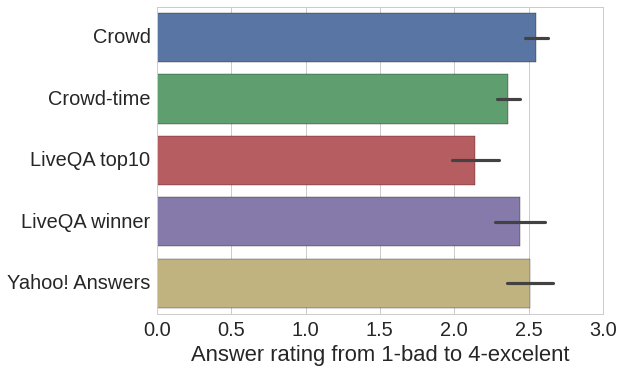
\includegraphics[width=0.5\textwidth]{img/average_score}
\caption{Average scores of different type of answers to Yahoo! Answers questions}
\label{fig:average_score}
\end{figure}

\begin{figure}[h]
\centering
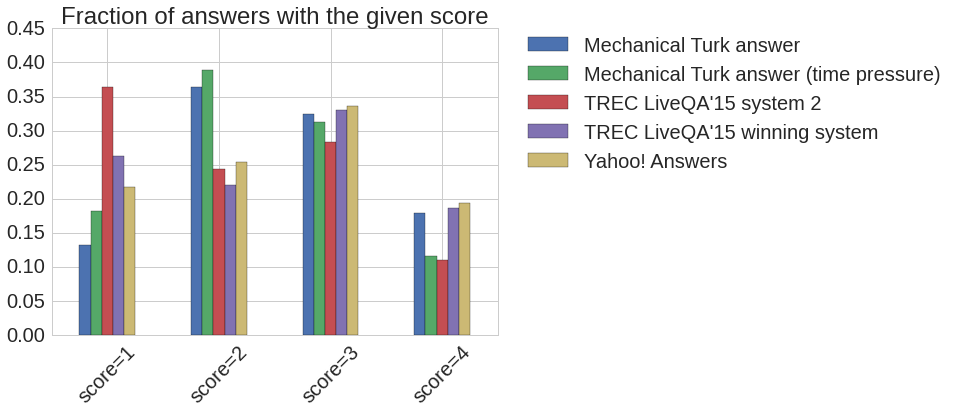
\includegraphics[width=0.5\textwidth]{img/scores_distribution}
\caption{Distribution of scores for different types of answers to Yahoo! Answers questions}
\label{fig:scores_distribution}
\end{figure}

\section{Discussion}
\label{sec:discussion}

Some discussion on the results and possible future work.

\section{Related Work}
\label{sec:related_work}

In \cite{bernstein2012direct} authors used a combination of log mining and crowdsourcing to build answers to a long tail of questions, that search engine users ask, therefore increasing the coverage of direct answers

\section{Conclusion}
\label{sec:conclusion}

Final words.

\section*{Acknowledgments}

If any...

\bibliography{naaclhlt2016}
\bibliographystyle{naaclhlt2016}


\end{document}
